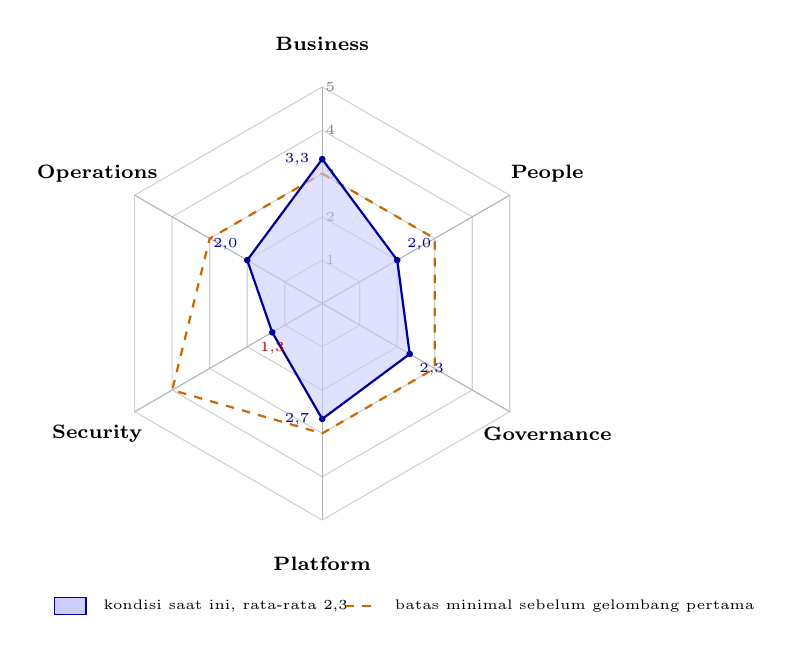
\begin{tikzpicture}[font=\scriptsize]
  % Satu satuan skor sama dengan 0,55 cm. Skala 1 sampai 5.
  \foreach \skor in {1,...,5} {
    \draw[gray!35] (90:{\skor*0.55}) -- (30:{\skor*0.55}) -- (-30:{\skor*0.55})
      -- (-90:{\skor*0.55}) -- (-150:{\skor*0.55}) -- (150:{\skor*0.55}) -- cycle;
    \node[gray, font=\tiny, anchor=west, inner sep=1pt] at (90:{\skor*0.55}) {\skor};
  }

  % Enam sumbu perspektif. Sisi kanan bisnis, sisi kiri teknis.
  \foreach \sudut/\nama in {90/Business, 30/People, -30/Governance,
    -90/Platform, -150/Security, 150/Operations} {
    \draw[gray!60] (0,0) -- (\sudut:2.75);
    \node[font=\scriptsize\bfseries] at (\sudut:3.3) {\nama};
  }

  % Batas minimal sebelum gelombang pertama: 3, kecuali Security 4.
  \draw[thick, dashed, orange!80!black] (90:1.65) -- (30:1.65) -- (-30:1.65)
    -- (-90:1.65) -- (-150:2.2) -- (150:1.65) -- cycle;

  % Kondisi saat ini, rata-rata tiga pertanyaan per perspektif.
  \draw[thick, draw=blue!60!black, fill=blue!20, fill opacity=0.6]
    (90:1.833) -- (30:1.1) -- (-30:1.283) -- (-90:1.467) -- (-150:0.733)
    -- (150:1.1) -- cycle;
  \foreach \sudut/\jarak in {90/1.833, 30/1.1, -30/1.283, -90/1.467,
    -150/0.733, 150/1.1} {
    \fill[blue!60!black] (\sudut:\jarak) circle (1.2pt);
  }
  \node[font=\tiny, blue!60!black, anchor=east] at (90:1.833) {3,3\,};
  \node[font=\tiny, blue!60!black, anchor=south west] at (30:1.1) {2,0};
  \node[font=\tiny, blue!60!black, anchor=north west] at (-30:1.283) {2,3};
  \node[font=\tiny, blue!60!black, anchor=east] at (-90:1.467) {2,7\,};
  \node[font=\tiny, red!70!black, anchor=north] at (-150:0.733) {1,3};
  \node[font=\tiny, blue!60!black, anchor=south east] at (150:1.1) {2,0};

  % Keterangan.
  \fill[blue!20, draw=blue!60!black] (-3.4,-3.95) rectangle ++(0.4,0.22);
  \node[anchor=west, font=\tiny] at (-2.9,-3.84) {kondisi saat ini, rata-rata 2,3};
  \draw[thick, dashed, orange!80!black] (0.3,-3.84) -- ++(0.4,0);
  \node[anchor=west, font=\tiny] at (0.8,-3.84)
    {batas minimal sebelum gelombang pertama};
\end{tikzpicture}
